\documentclass[12pt,a4paper]{article}
\usepackage[utf8]{inputenc}
\usepackage[french]{babel}
\usepackage[T1]{fontenc}
\usepackage{amsmath}
\usepackage{amsfonts}
\usepackage{amssymb}
\usepackage{graphicx}
\usepackage[left=2cm,right=2cm,top=2cm,bottom=2cm]{geometry}
%\author{Rémi Metzdorff}
\title{Utilisation d'un réseau en spectroscopie}

\usepackage{xcolor}
\definecolor{theme}{RGB}{56,115,179}

\usepackage{hyperref}
\hypersetup{
    colorlinks=true,
    linkcolor=red,
    filecolor=green,      
    urlcolor=theme,
}

\renewcommand{\d}{\mathrm{d}}


\begin{document}
\maketitle

\section*{Introduction}

Grâce à leur pouvoir de dispersion important, les réseaux sont beaucoup utilisés en spectroscopie afin de caractériser différents rayonnement.
On en retrouve dans les spectromètres et le monochromateur par exemple.
Associés à une diode laser, ils permettent d'obtenir simplement des lasers accordables : diode en cavité étendue.

Un exemple un peu original : le spectromètre à réseau de transmission de haute énergie du télescope spatial Chandra.

\section{Objectif de la manipulation}

\begin{figure}[!b]
\center
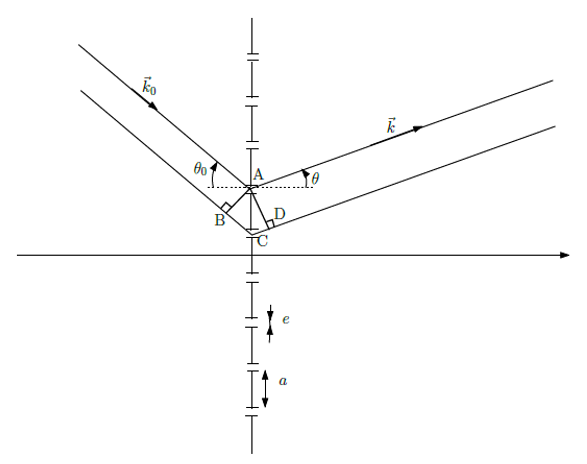
\includegraphics[height=200pt]{reseau.png}
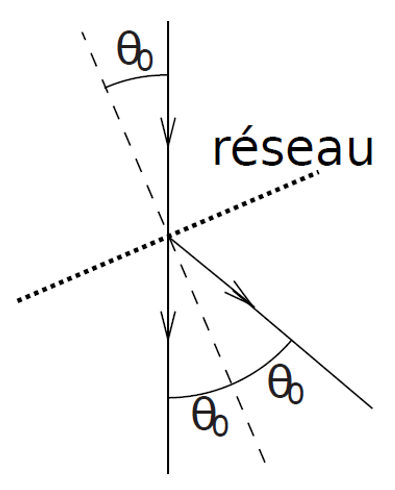
\includegraphics[height=200pt]{reseau_min.png}
\caption{Schéma de la diffraction par un réseau et configuration au minimum de déviation.}
\label{fig:reseau}
\end{figure}

L'objectif est d'analyser la lumière issue d'une source donnée à l'aide d'un réseau.
La lumière transmise par un réseau est dispersée : chaque longueur d'onde est associée à un angle de déviation qui dépend du pas du réseau, de l'ordre de diffraction et de l'angle incident.
On peut se placer au minimum de déviation, configuration particulière pour laquelle $\theta = -2\theta_0$ (voir Fig.~\ref{fig:reseau} pour les notations).
Dans ce cas, la déviation $D_m$ vaut $2\theta_0$ et le lien avec la longueur d'onde est simplement $2a\sin\theta_0=p\lambda$, où $a$ est le pas du réseau, $p$ l'ordre de diffraction et $\lambda$ la longueur d'onde.

\section{Aspect théorique}

On utilise les notations de la Fig.~\ref{fig:reseau} et on suppose pour simplifier que le réseau est parfaitement diffractant, c'est-à-dire que $e \rightarrow 0$.
On ne s'intéresse pas ici aux détails de la figure de diffraction mais l'expression complète est donnée dans le TD de Clément Sayrin \href{http://www.lkb.upmc.fr/cqed/wp-content/uploads/sites/14/2019/10/optique_TD_diffraction_1_corrige.pdf}{Diffraction (1)}.
On compte positivement les angles orientés dans le sens trigonométrique.
On se place dans les conditions de Fraunhofer.

La différence de marche $\delta$ entre les deux faisceaux issus de deux fentes successives est
\begin{equation}
\delta = n_\mathrm{air}(BC+CD).
\end{equation}
En prenant $n_\mathrm{air}=1$ et avec un peu de trigonométrie dans les triangles rectangles $ABC$ et $ADC$, on obtient
\begin{equation}
\delta = a(-\sin\theta_0 + \sin\theta).
\end{equation}
Pour que l'intensité diffractée dans le direction $\theta$ soit maximale, il faut qu'il y ait interférence constructive, c'est-à-dire que les ondes soient en phase, soit $\delta=p\lambda$ où $p$ est un entier.
On obtient finalement la formule des réseaux :
\begin{equation}
\sin\theta = p\frac{\lambda}{a} + \sin\theta_0
\label{eq:reseau}
\end{equation}

La déviation $D$ s'exprime $D=\theta-\theta_0$ et le minimum de déviation $D_m$ est atteint si $\d D = 0$ soit
\begin{equation}
\d\theta = \d\theta_0.
\end{equation}
En différenciant la relation \eqref{eq:reseau}, on trouve que cette condition est équivalente à $\theta=-\theta_0$ d'où $D_m = 2\theta$ (la solution $\theta=\theta_0$ correspond à $D=0$ et n'est pas intéressante puisqu'alors, le faisceau n'est pas dévié).
En utilisant la formule des réseaux on trouve finalement
\begin{equation}
\sin\left(\frac{D_m}{2}\right) = p\frac{\lambda}{2a}.
\end{equation}
La mesure de l'angle minimum de déviation permet donc de remonter à la longueur d'onde de la lumière analysée si le pas du réseau est connu.
Inversement, on peut caractériser un réseau à partir d'un rayonnement connu.

\section{Manipulation}

\begin{figure}
\center
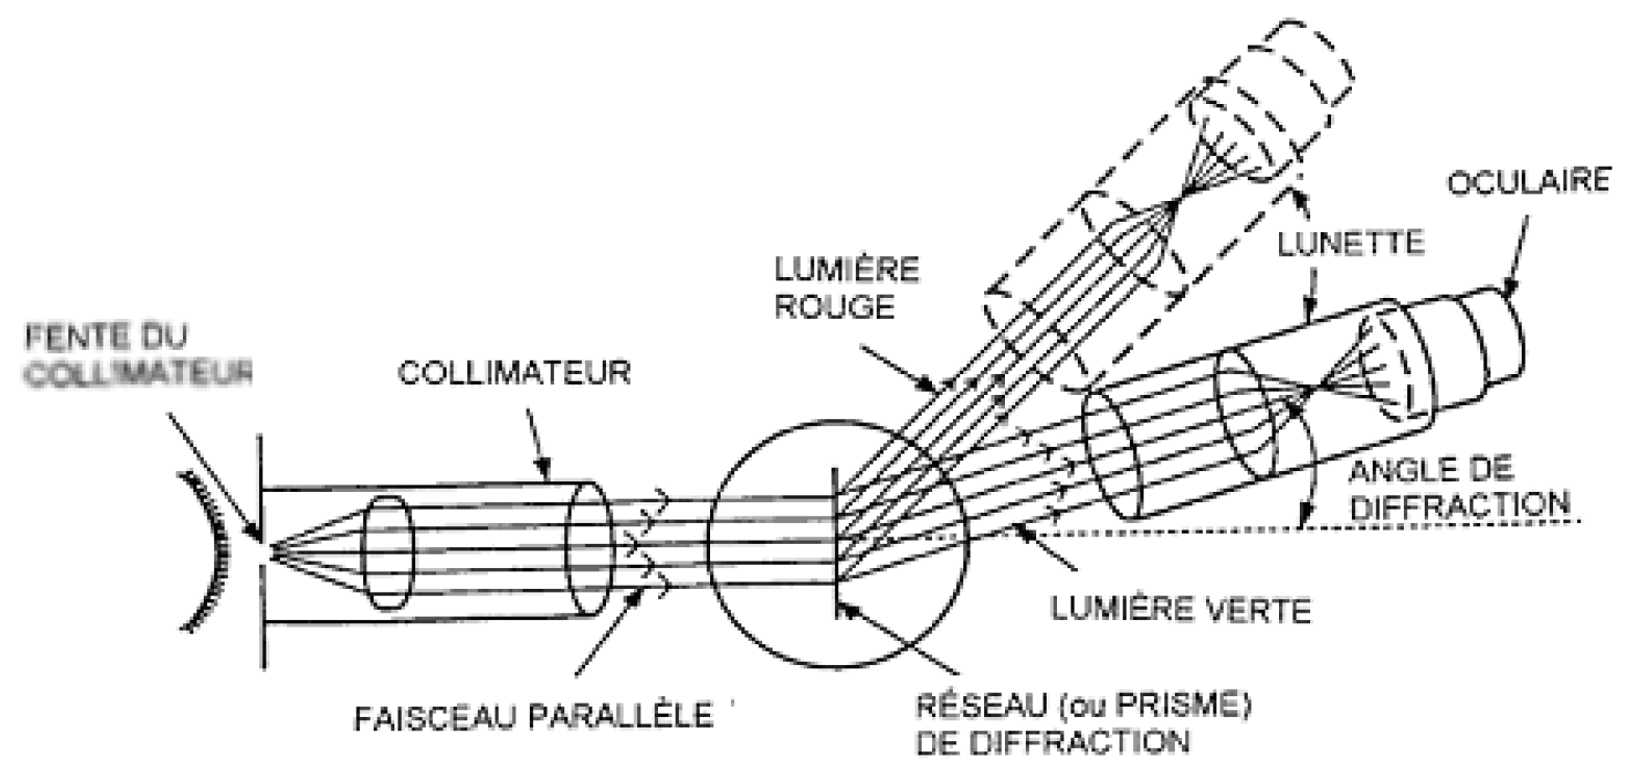
\includegraphics[height=200pt]{goniometre.png}
\caption{Schéma de principe d'un goniomètre.}
\label{fig:gonio}
\end{figure}

Une vidéo sur le \href{https://www.youtube.com/watch?v=oj9gK-VMGg8}{réglage du goniomètre} et sur la \href{https://www.youtube.com/watch?v=L8cT_YwTXzI}{manipulation}.

On peut mesurer les raies d'émission d'une lampe spectrale Hg Zn Cd par exemple.
\begin{enumerate}
\item Régler le goniomètre (Fig.~\ref{fig:gonio}) : voir le \href{http://ressources.agreg.phys.ens.fr/static/TP/serie3/Spectroscopie.pdf}{polycopié de TP}.
\item Mesurer le minimum de déviation pour une raie donnée d'un côté du goniomètre puis de l'autre.
\item Répéter pour quelques raies.
\end{enumerate}
On peut faire cette mesure avec un prisme mais son pouvoir dispersif est moindre.
La meilleure précision est obtenue pour un réseau avec un grand nombre de traits par millimètre : $D_m$ est d'autant plus grand que $a$ est faible.

\section{Interprétation}

Comparer les valeurs obtenues avec celles indiquées dans la \href{https://agreg.phys.ens.fr/notices/N0102.pdf}{notice}.
On peut aussi se référer au \href{https://physics.nist.gov/PhysRefData/ASD/lines_form.html}{site du NIST} qui répertorie toutes les raies d'émission connues.

On doit pouvoir aussi faire la spectroscopie de la lampe de Balmer pour vérifier la formule de Rydberg donnant les énergies de transition de l'hydrogène.

\section{Incertitudes}

Les incertitudes portent sur le pas du réseau $a \pm u_a$ et sur la détermination de l'angle de déviation minimum $D_m \pm u_{D_m}$.
Il n'y a pas d'incertitude sur $p$ sous réserve que l'on ne se trompe pas d'ordre de diffraction.
On a 
\begin{equation}
\lambda = \frac{2a}{p} \sin\left(\frac{D_m}{2}\right)
\end{equation}
que l'on différencie pour la propagation des incertitudes :
\begin{equation}
\d \lambda = \frac{2}{p} \sin\left(\frac{D_m}{2}\right) \d a + \frac{a}{p} \cos\left(\frac{D_m}{2}\right) \d D_m.
\end{equation}
On élève chaque terme au carré et on obtient la formule de propagation des incertitudes :
\begin{equation}
u_\lambda = \sqrt{ \left[\frac{2}{p} \sin\left(\frac{D_m}{2}\right)\right]^2 u_a^2 + \left[\frac{a}{p} \cos\left(\frac{D_m}{2}\right)\right]^2 u_{D_m}^2 }.
\end{equation}

En mesurant l'angle de déviation minimum deux fois (de chaque côté de l'axe du goniomètre), on peut prendre la moyenne et l'incertitude est réduite d'un facteur $1/\sqrt{2}$.
Attention à bien mettre les incertitudes sur les angles en radian !

\section*{Conclusion}

Sinon on utilise directement un spectromètre fibré qui est déjà calibré...
En tous cas on peut utiliser le spectromètre pour comparer les valeurs aussi.

\end{document}